\subsection{Metodología}
\subsubsection{Metodología Tecnológica}

La metodología usada para el desarrollo se ha basado en la investigación de las soluciones descentralizadas ya que el objetivo es crear una infraestructura que promoviera la descentralización y la trazabilidad de los activos.

\bigskip

También se destaca  la Stack tecnológica,\footnote{Conjunto de herramientas y arquitecturas usadas para el desarrollo de software.} ya que esta varia drásticamente de la común, esto se debe a que los Smart Contracts eliminan la necesidad de tener una arquitectura Back-end clásica, mientras que la blockchain con la que interactúan reemplaza el uso de una base de datos.

\begin{figure}[H]
        \centering
        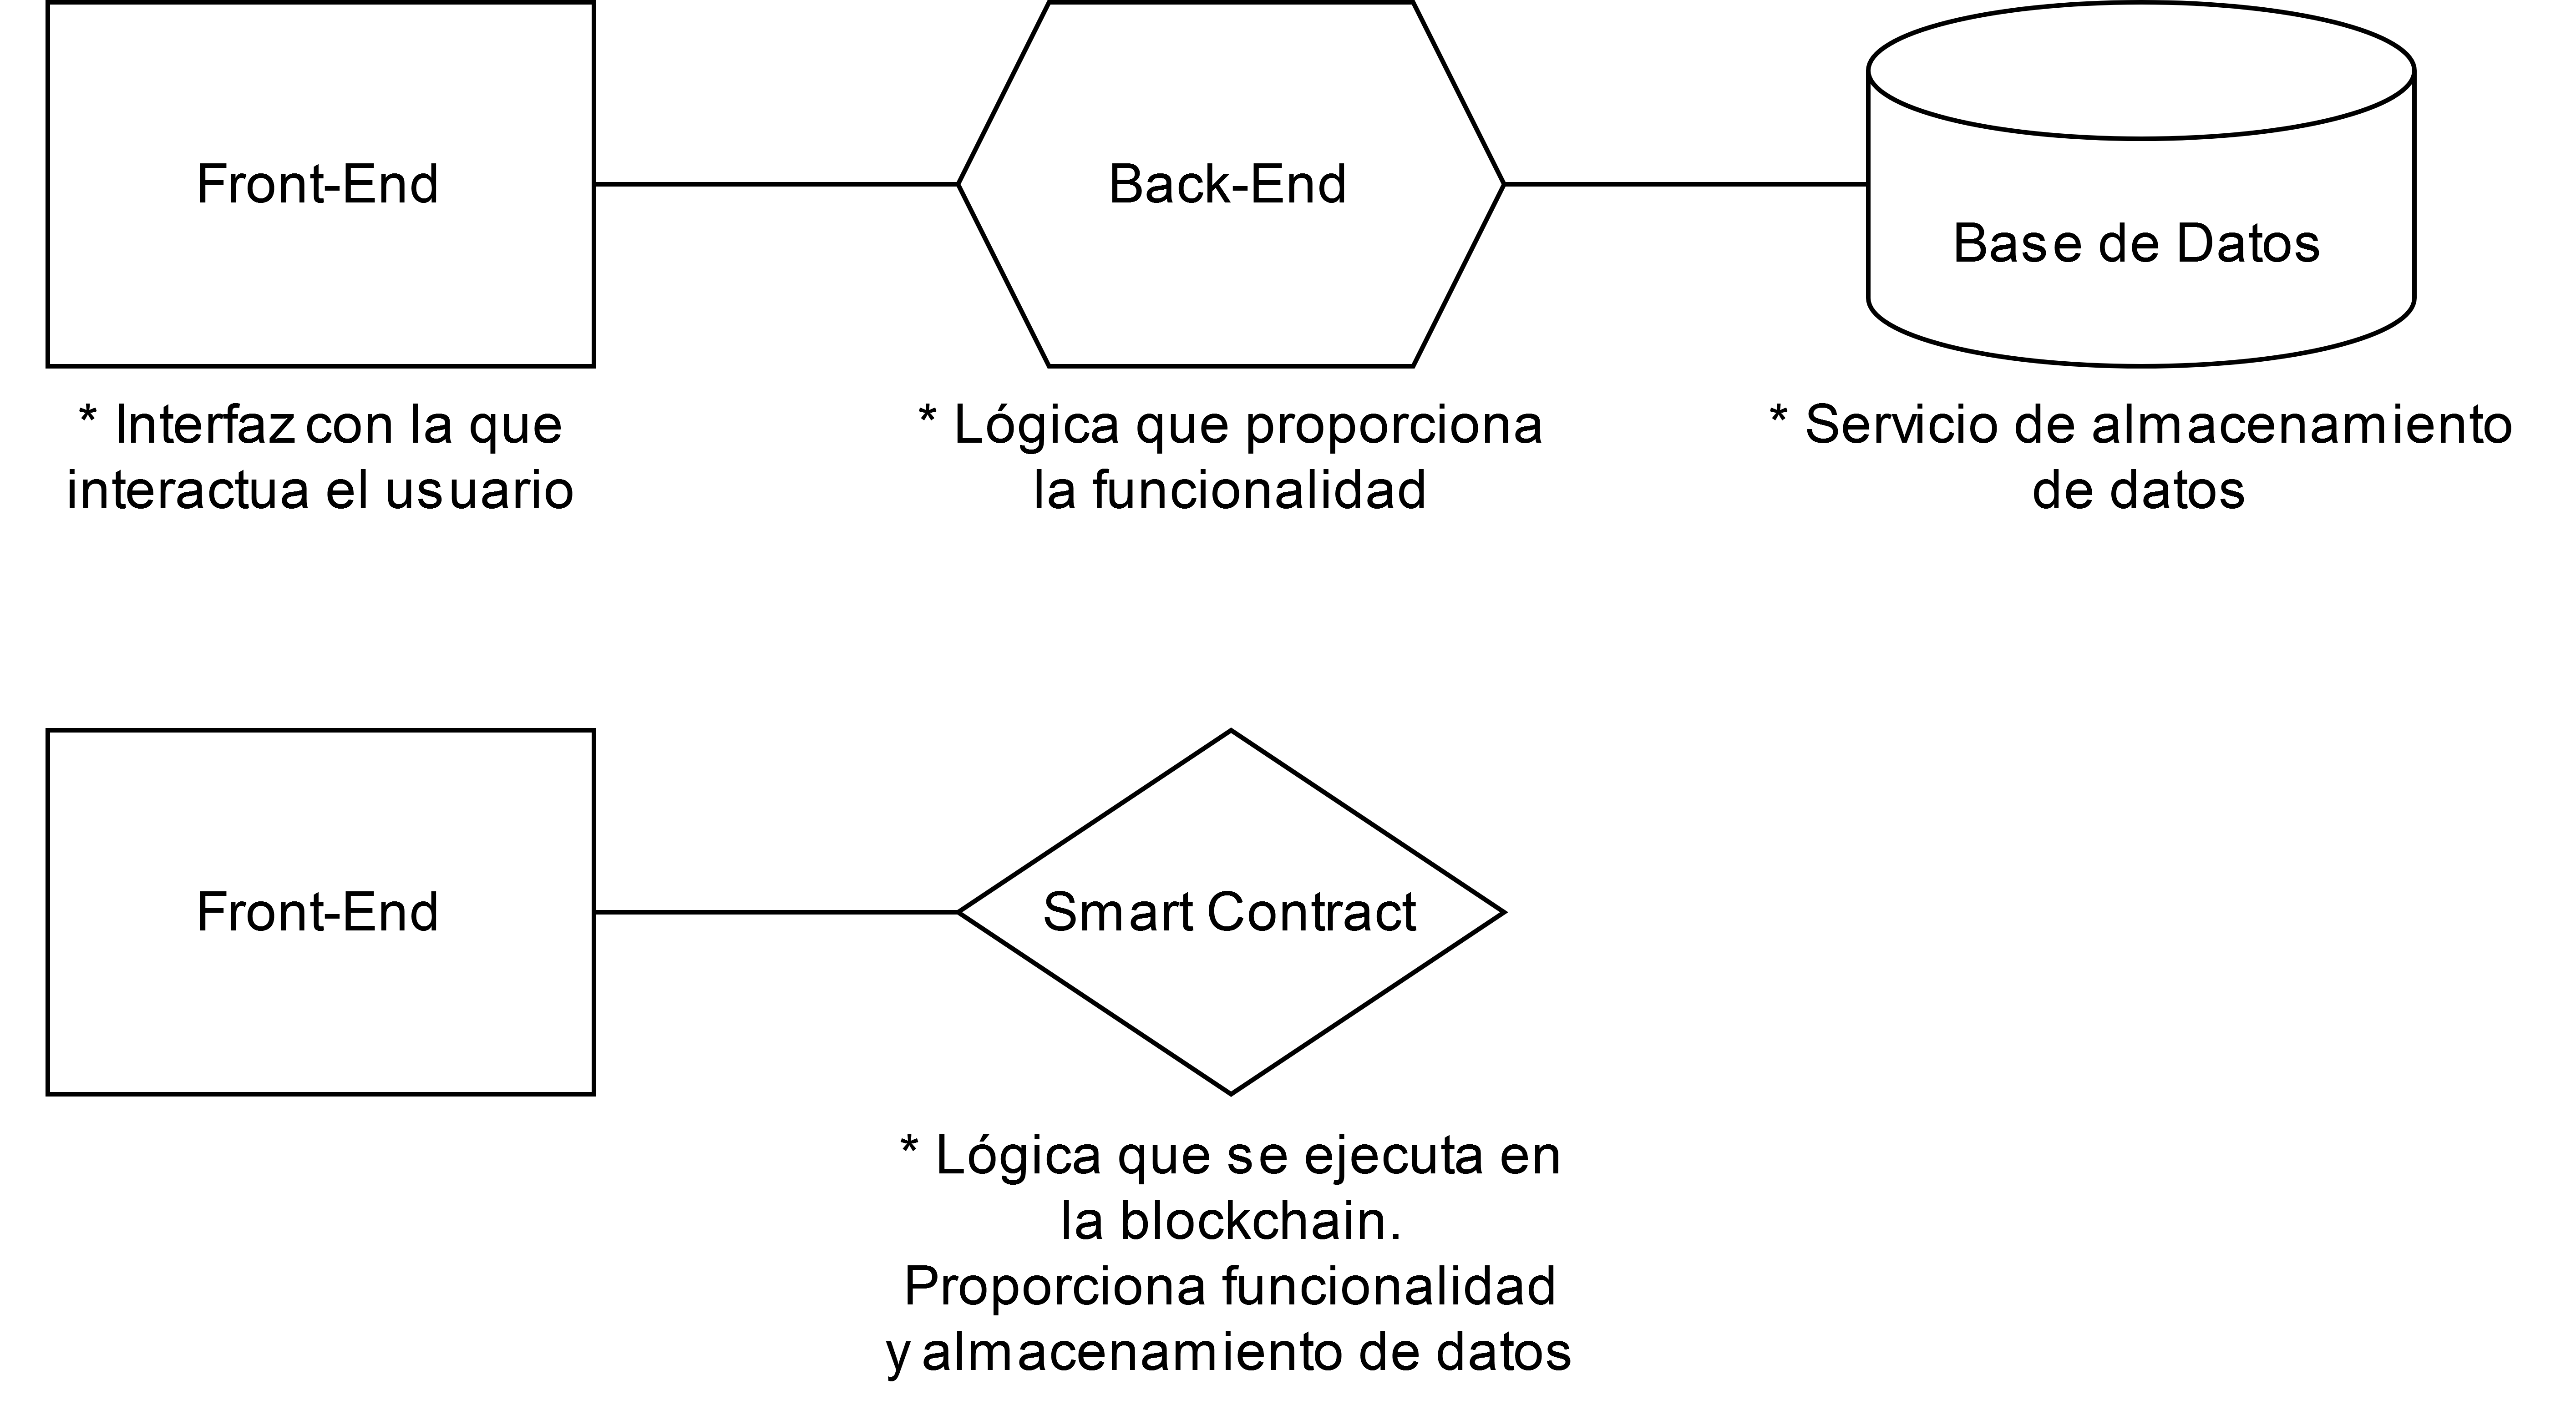
\includegraphics[width=0.8\textwidth]{img/diagramas/metodologia.png}
        \caption{Comparativa entre la arquitectura común Cliente-Servidor-DB y Cliente-Smart Contract.}
        \label{fig:configApi}
\end{figure}

\bigskip

Para el desarollo de este sistema, se hace uso de Hardhat, un framework que permite el despliegue de una red blockchain local simulada usando el protocolo Ethereum para el desarrollo, testeo y despliegue de los smart contracts a la red de Polygon, Svelte para el desarrollo ágil de un front-end usando JavaScript, Bootstrap para dotar de un estilo user-friendly\footnote{Diseño o sistema que es fácil de usar y entender por los usuarios, lo que facilita su interacción y mejora su experiencia.} al front-end, la librería EthersJS para interconectar el front-end con los smart contracts, y la librería ThirdWeb para interconectarnos con la blockchain IPFS para el almacenamiento de imágenes, vídeos y otros archivos.

\subsubsection{Metodología de Desarrollo}

Durante la implementación se ha usado la metodología ágil para planificar la implementación de la aplicación por partes, pero con una gran flexibilidad ya que el equipo solo está formado por una persona. 

\bigskip

Se usa CI mediante \textcolor{blue}{\href{https://github.com/features/actions}{\textbf{Github Actions}}}\footnote{\url{https://github.com/features/actions}} para poder realizar los tests en el Smart Contract ( mediante MochaJS ) y desplegar de forma automática mediante DockerHub la interfaz web.